\documentclass[tikz,border=7pt]{standalone}
\usepackage{amsmath,amssymb}
\usepackage[scaled]{helvet}
\renewcommand{\familydefault}{\sfdefault}
\usetikzlibrary{arrows.meta,backgrounds,calc,fit,positioning,shapes.geometric}
\definecolor{bpink}{HTML}{172033}
\definecolor{bpblue}{HTML}{2A78D6}
\definecolor{bporange}{HTML}{E56A32}
\definecolor{bpgreen}{HTML}{168A65}
\definecolor{bppurple}{HTML}{7A5CC7}
\definecolor{bpred}{HTML}{C94A4A}
\definecolor{bpmuted}{HTML}{667085}
\definecolor{bpgrid}{HTML}{D8DEE8}
\definecolor{bpsurface}{HTML}{F8FAFC}
\tikzset{
  var/.style={circle,draw=bpblue,fill=bpblue!10,line width=.9pt,minimum size=8mm,font=\small\bfseries,text=bpink},
  factor/.style={rectangle,rounded corners=1.5pt,draw=bporange,fill=bporange!14,line width=.9pt,minimum size=6.8mm,font=\small\bfseries,text=bpink},
  constraint/.style={rectangle,rounded corners=1.5pt,draw=bpred,fill=bpred!12,line width=.9pt,minimum size=6.8mm,font=\small\bfseries,text=bpink},
  edge/.style={draw=bpmuted!75,line width=.9pt},
  msgvf/.style={-{Latex[length=2.2mm]},draw=bpblue,line width=1.35pt},
  msgfv/.style={-{Latex[length=2.2mm]},draw=bporange,line width=1.35pt},
  label/.style={font=\scriptsize,text=bpmuted,align=center},
  title/.style={font=\bfseries\large,text=bpink},
  card/.style={draw=bpgrid,fill=bpsurface,rounded corners=7pt,line width=.7pt},
}

\begin{document}
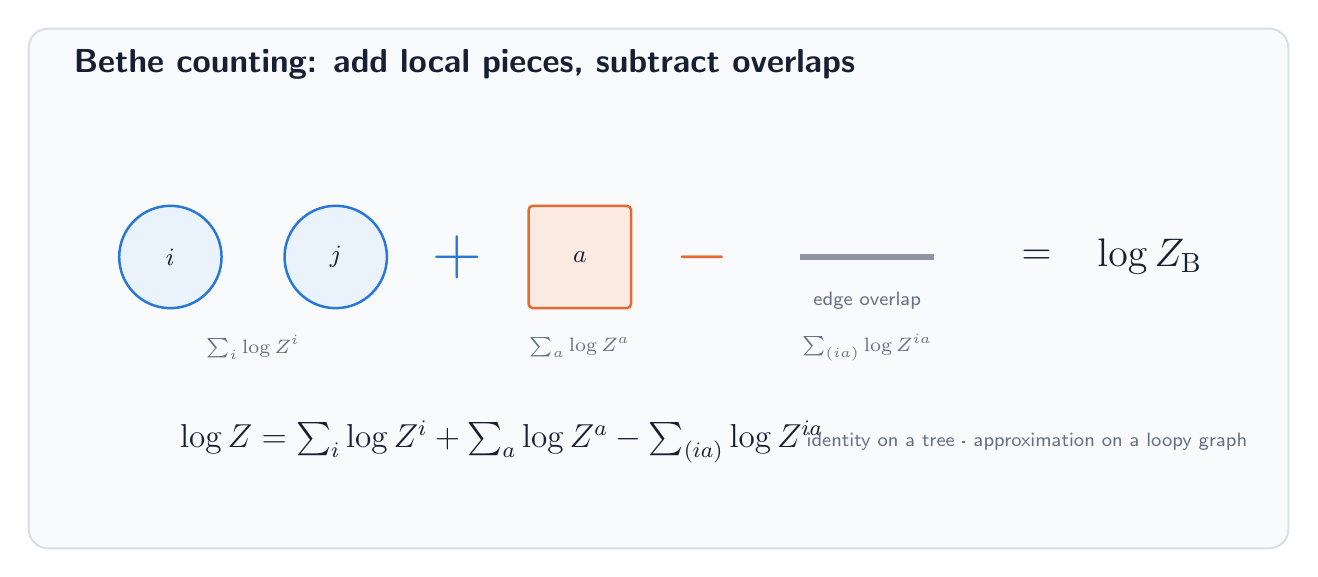
\begin{tikzpicture}[font=\sffamily]
  \node[card,minimum width=16cm,minimum height=6.6cm] at (7.2,2.1) {};
  \node[title,anchor=west] at (-.35,4.95) {Bethe counting: add local pieces, subtract overlaps};
  \node[var,minimum size=13mm] (i) at (1.0,2.5) {$i$};
  \node[var,minimum size=13mm] (j) at (3.1,2.5) {$j$};
  \node[text=bpblue,font=\Huge\bfseries] at (4.65,2.5) {$+$};
  \node[factor,minimum size=13mm] (a) at (6.2,2.5) {$a$};
  \node[text=bporange,font=\Huge\bfseries] at (7.75,2.5) {$-$};
  \draw[edge,line width=2.4pt] (9.0,2.5)--(10.7,2.5);
  \node[text=bpmuted,font=\scriptsize] at (9.85,1.95) {edge overlap};
  \node[text=bpink,font=\Large] at (12.0,2.5) {$=$};
  \node[anchor=west,text=bpink,font=\Large] at (12.65,2.5) {$\log Z_{\mathrm B}$};
  \node[label] at (2.05,1.35) {$\sum_i\log Z^i$};
  \node[label] at (6.2,1.35) {$\sum_a\log Z^a$};
  \node[label] at (9.85,1.35) {$\sum_{(ia)}\log Z^{ia}$};
  \node[anchor=west,text=bpink,font=\large] at (1.0,.15) {$\log Z=\sum_i\log Z^i+\sum_a\log Z^a-\sum_{(ia)}\log Z^{ia}$};
  \node[anchor=east,label] at (14.8,.15) {identity on a tree · approximation on a loopy graph};
\end{tikzpicture}
\end{document}
